\documentclass[10pt]{article}

\usepackage{amsmath}
\usepackage{fullpage}
\usepackage{array}
\usepackage{graphicx}
\usepackage{gensymb}
\usepackage{booktabs}
\usepackage{gensymb}
\usepackage{graphicx}

\graphicspath{ {../Images/} }

\date{2014-6-22}
\pagestyle{empty}
\setlength{\parindent}{0pt}

\begin{document}
\begin{center}
\begin{Large}\textbf{Physical Science 303 - Extra Credit Assignment}\end{Large} \\
\smallskip
%\begin{large} Acceleration \end{large}
\end{center}
%%%%%%%

 \begin{enumerate}
\item Find the acceleration (magnitude and direction) of the mass $m=3$ kg sliding on a fixed inclined plane with the $\theta=30^\circ$ as shown in figure.  Compute the acceleration for $\mu_k=0$ (frictionless) and $\mu_k=0.1$.
\begin{figure}[h]
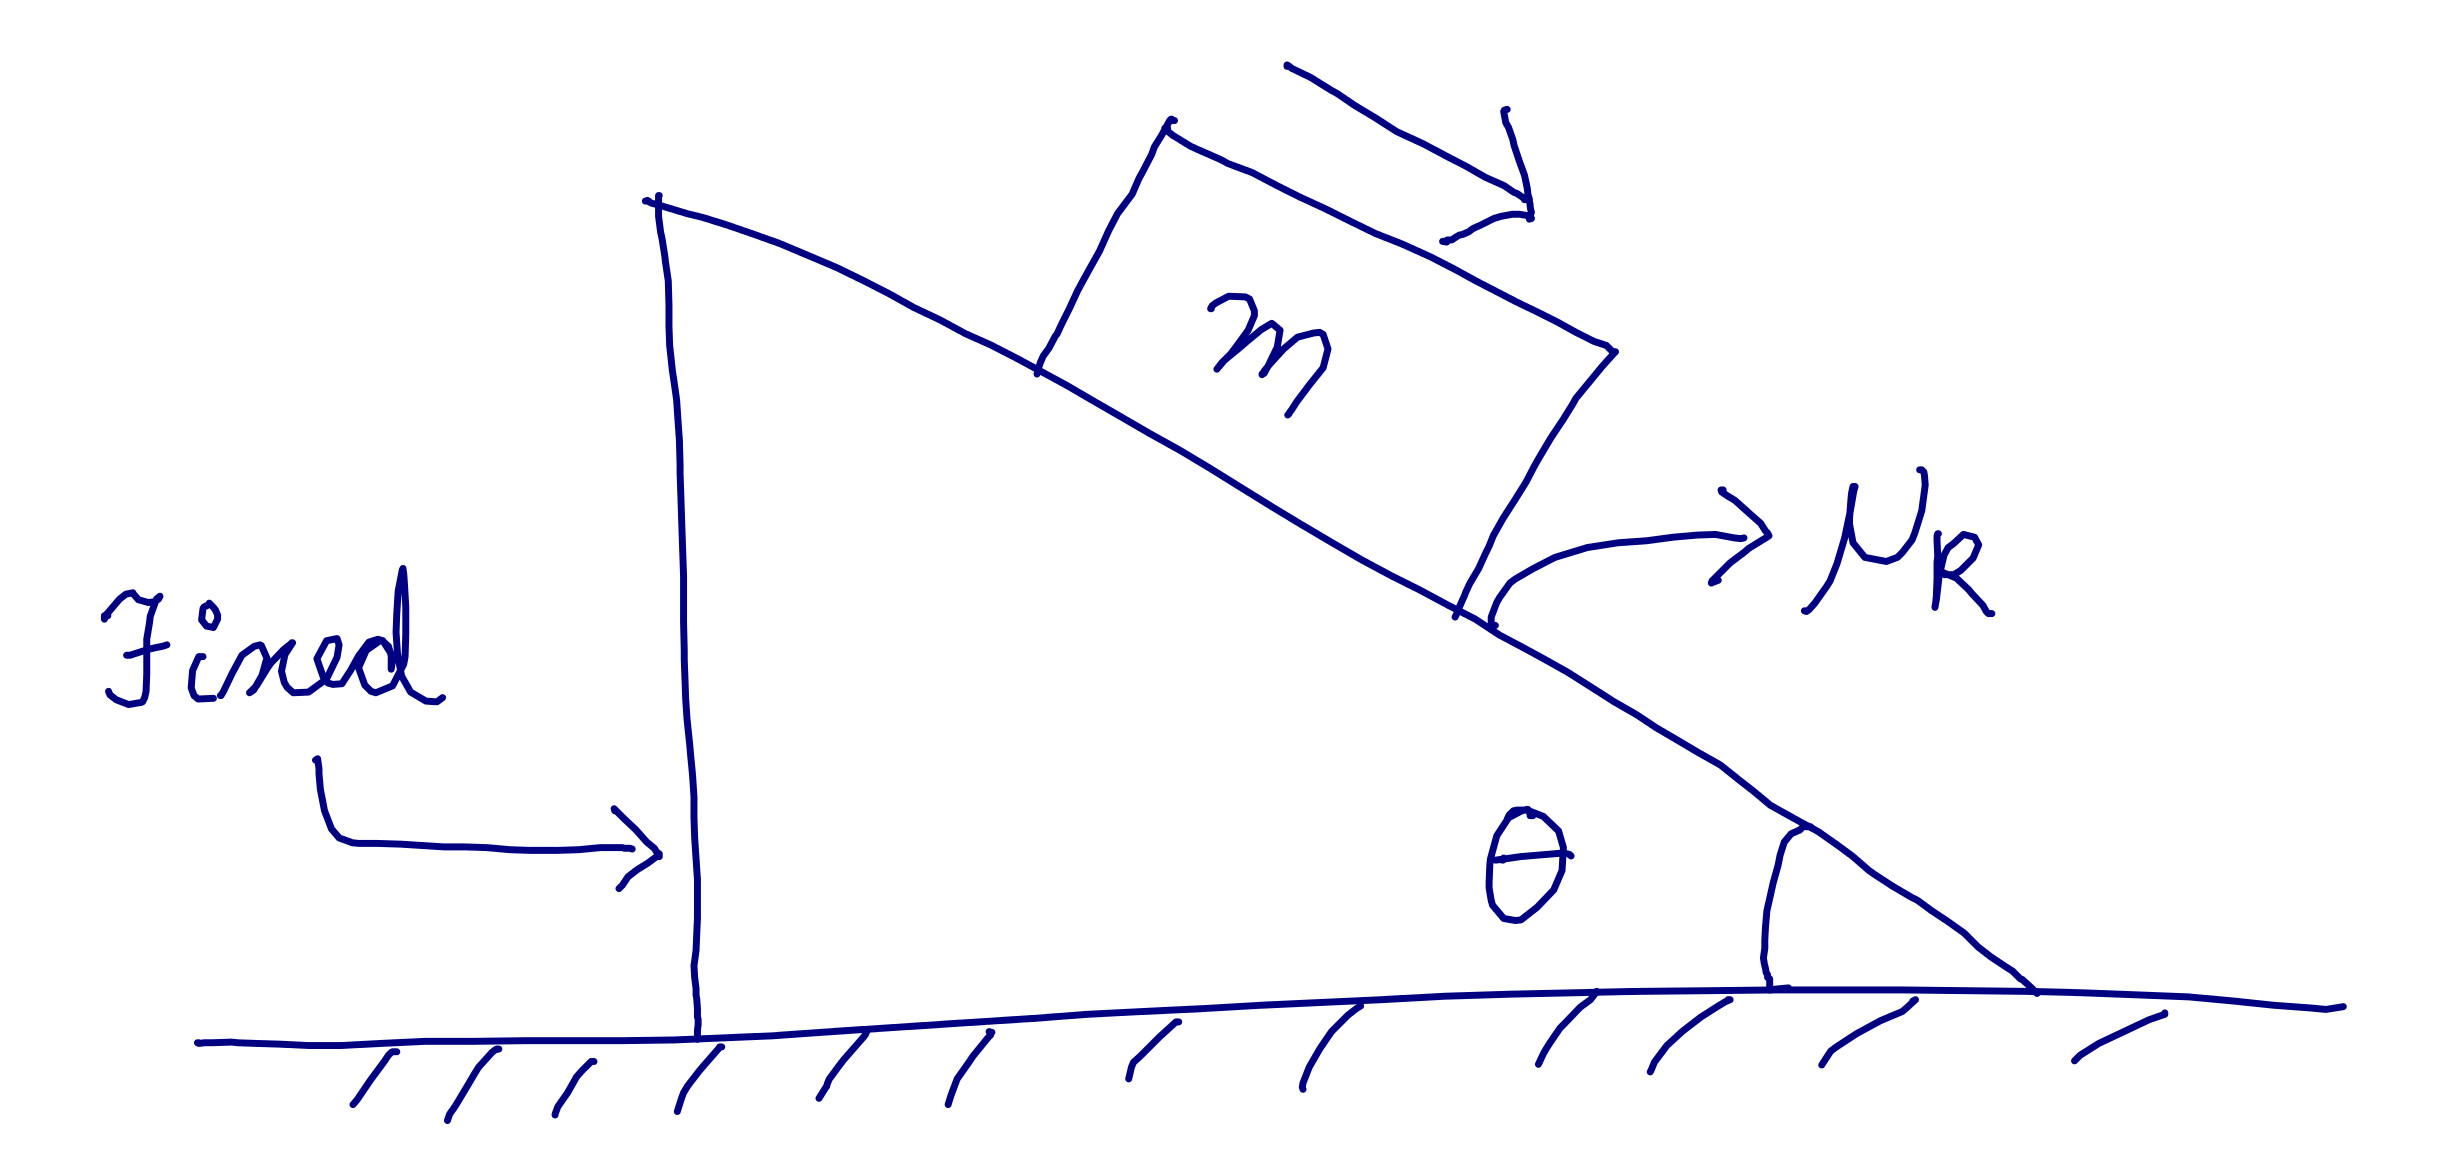
\includegraphics[scale=.5]{inclinedextra}
\centering
\end{figure}\\
Directions: As usual, draw the FBD for the mass (consider all the possible forces acting on it).  Choose a convenient set of axis and resolve the forces along them.  Finally apply the Newton's laws of motion for both the axis and find the resultant motion of the mass.
\end{enumerate}
\end{document}
